\documentclass[mathserif,compress]{beamer} 
\usepackage{pdfpages}
%\usepackage{handoutWithNotes} 
%\pgfpagesuselayout{4 on 1 with notes}[a4paper, border shrink=5mm]
%\pgfpageslogicalpageoptions{1}{border code=\pgfusepath{stroke}}
%\pgfpageslogicalpageoptions{2}{border code=\pgfusepath{stroke}}
%\pgfpageslogicalpageoptions{3}{border code=\pgfusepath{stroke}}
%\pgfpageslogicalpageoptions{4}{border code=\pgfusepath{stroke}}

\usepackage{beamerthemeDresden} 
\usepackage[english]{babel}
\usepackage{amsmath,amssymb}
\usepackage[latin1]{inputenc}
\usepackage{palatino}
\usepackage{graphicx}
\usepackage{subfigure}
\usepackage{pgf}
\usepackage{relsize}
\usepackage{tabularx}
\usepackage{setspace}
%\beamertemplateshadingbackground{red!1}{blue!1}
% Use some nice templates
\beamertemplatetransparentcovereddynamic  


\def\beq{\begin{equation}}
\def\eeq{\end{equation}}
\def\bit{\begin{itemize}}
\def\eit{\end{itemize}}
\def\bdm{\begin{displaymath}}
\def\edm{\end{displaymath}}
\def\ben{\begin{enumerate}}
\def\een{\end{enumerate}}
\def\bc{\mathbf{c}}
\def\be{\mathbf{e}}
\def\bh{\mathbf{h}}
\def\bn{\mathbf{n}}
\def\br{\mathbf{r}}
\def\bs{\mathbf{s}}
\def\bu{\mathbf{u}}
\def\bw{\mathbf{w}}
\def\bx{\mathbf{x}}
\def\by{\mathbf{y}}
\def\bz{\mathbf{z}}
\def\bA{\mathbf{A}}
\def\bB{\mathbf{B}}
\def\bC{\mathbf{C}}
\def\bD{\mathbf{D}}
\def\bG{\mathbf{G}}
\def\bI{\mathbf{I}}
\def\bM{\mathbf{M}}
\def\bP{\mathbf{P}}
\def\bQ{\mathbf{Q}}
\def\bR{\mathbf{R}}
\def\bS{\mathbf{S}}
\def\bV{\mathbf{V}}
\def\bW{\mathbf{W}}
\def\bX{\mathbf{X}}
\def\bY{\mathbf{Y}}
\def\bZ{\mathbf{Z}}
\def\cB{\mathcal{B}}
\def\cF{\mathcal{F}}
\def\cI{\mathcal{I}}
\def\cK{\mathcal{K}}
\def\cU{\mathcal{U}}
\def\balpha{\mbox{\boldmath $\alpha$}}
\def\bbeta{\mbox{\boldmath $\beta$}}
\def\bepsilon{\mbox{\boldmath $\epsilon$}}
\def\bdelta{\mbox{\boldmath $\delta$}}
\def\bgamma{\mbox{\boldmath $\gamma$}}
\def\bldeta{\mbox{\boldmath $\eta$}}
\def\bphi{\mbox{\boldmath $\phi$}}
\def\bkappa{\mbox{\boldmath $\kappa$}}
\def\blambda{\mbox{\boldmath $\lambda$}}
\def\bmu{\mbox{\boldmath $\mu$}}
\def\bnu{\mbox{\boldmath $\nu$}}
\def\btheta{\mbox{\boldmath $\theta$}}
\def\brho{\mbox{\boldmath $\rho$}}
\def\bDelta{\mbox{\boldmath $\Delta$}}
\def\bLambda{\mbox{\boldmath $\Lambda$}}
\def\bSigma{\mbox{\boldmath $\Sigma$}}
\def\var{\textrm{var}}
\def\cov{\textrm{cov}}
\def\log{\textrm{log}}
\def\median{\textrm{median}}
\def\argmin{\textrm{arg min }}
\def\bzero{\mathbf{0}}
\def\bone{\mathbf{1}}
\def\Poi{\textrm{Poi}}
\def\Unif{\textrm{Unif}}
\def\upp{^{\prime}}
\def\upi{^{-1}}
\newcommand{\cye}[1]{\color{yellow!70!black}#1}
\newcommand{\cre}[1]{\color{red!70!black}#1}
\newcommand{\cbl}[1]{\color{blue!70!black}#1}
\newcommand{\cgr}[1]{\color{green!70!black}#1}
\newcommand{\cpu}[1]{\color{blue!65!red}#1}
\newcommand{\fsz}[1]{{\footnotesize #1}}
\newcommand{\ssz}[1]{{\scriptsize #1}}

%-------------------------------------------------------------------------------

\title[]{A Quick and Dirty Bayesian Leslie Matrix Model of Norway HarpEast Data }

\author[Jay M. Ver Hoef]{Jay Ver Hoef} 

\institute[Marine Mammal Laboratory]
{
	\normalsize Marine Mammal Laboratory \\
	NOAA Fisheries Alaska Science Center \\
	Seattle, Washington and Fairbanks, Alaska, USA\\
	\vspace{0.1cm}
}
\date[11/06/20]{}
%-------------------------------------------------------------------------------
\begin{document}

%-------------------------------------------------------------------------------
\frame{\titlepage}
%-------------------------------------------------------------------------------

%-----------------------------------------------------------------------
%           The Model
%-----------------------------------------------------------------------
\begin{frame} 
\vspace{-.5cm}

Population Values 

\vspace{.2cm}
$A_{t} = \textrm{Number of Nonpups in year } t$ \\
$H^{A}_{t} = \textrm{Harvest of Nonpups in year } t$ \\
$P_{t} = \textrm{Number of Pups in year } t$ \\
$H^{P}_{t} = \textrm{Harvest of Pups in year } t$ \\
$N_{t} = A_{t} + P_{t}$ \\

\end{frame}


%-----------------------------------------------------------------------
%           The Model
%-----------------------------------------------------------------------
\begin{frame} 
\vspace{-.5cm}
A Simple Two-age Leslie Matrix Model

\vspace{.2cm}

{\tiny 
\begin{singlespace}
 Boveng, P.L., Ver Hoef, J.M., Withrow, D.E., and London, J.M. 2018. A Bayesian Analysis of Abundance, Trend and Population Viability for Harbor Seals in Iliamna Lake, Alaska. Risk Analysis 38(9): 1988-209 DOI:10.1111/risa.12988
\end{singlespace}
}

$$
  \begin{tabular}{l}
    $A_t = \delta_{t-1}(A_{t-1}-H^{A}_{t-1}) + \kappa_{t-1}(P_{t-1} - H^{P}_{t-1})$, \\
		$P_t = c_{t-1}\phi_{t-1}(A_{t-1}-H^{A}_{t-1})$,
  \end{tabular}
$$

$$
  \bn_t = \left(\begin{array}{c}
    P_t \\
    A_t \\
  \end{array}\right), \
  \bh_t = \left(\begin{array}{c}
    H^{A}_t \\
    H^{P}_t \\
  \end{array}\right), \
  \bM_t = \left( \begin{array}{ll}
      0 & c_t\phi_t \\
      \kappa_t & \delta_t
  \end{array} \right)
$$

$$
\bn_{t} = \left(\bn_{t-1} - \bh_{t-1}\right) \bM_{t-1}
$$
$c_{t} = \exp(-\rho N_{t}/1000)$ 
$c_{t} = \textrm{Exponential decay in fecundity with increased } N_{t}$ 

\end{frame}

%-----------------------------------------------------------------------
%           Priors
%-----------------------------------------------------------------------
\begin{frame} 
Parameters

$P_{1}:\textrm{ Abundance of Pups in Year }t = 1$
$A_{1}:\textrm{ Abundance of Nonpups in Year }t = 1$
$\delta_{t}:\textrm{ Adult Mortality Rate in Year }t$
$\kappa_{t}:\textrm{ Pup Mortality Rate, from Survey to Survey, in Year }t$
$\phi_{t}:\textrm{ Fecundity Rate for all Adults, to Survey Time, in Year }t$
$\rho:\textrm{ Controls Exponential Decay in Fecundity as Population }\uparrow$

Priors

$[P_{1}] = \pi(P_{1}) \sim \textrm{N}(\textrm{300,000}, \hspace{.2cm} \textrm{50,000}^{2})$ \\
$[A_{1}] = \pi(A_{1}) \sim \textrm{N}(\textrm{1,000,000}, \hspace{.2cm} \textrm{100,000}^{2})$
$[\bdelta] = \pi(\textrm{logit}(\delta_{t})) \sim \textrm{N}(2.2, 0.5^{2}) \ \forall \ t; \ \textrm{logit}^{-1}(2.2) = 0.90$
$[\bkappa] = \pi(\textrm{logit}(\kappa_{t})) \sim \textrm{N}(1.4, 0.5^{2}) \ \forall \ t; \ \textrm{logit}^{-1}(1.4) = 0.80$
$[\bphi] = \pi(\textrm{logit}(\phi_{t})) \sim \textrm{N}(-0.4, 0.5^{2}) \ \forall \ t; \textrm{logit}^{-1}(-0.4) = 0.40$
$[\rho] = \pi(\textrm{log}(\rho)) \sim \textrm{N}(-4.0, 0.5^{2})$ \\


\end{frame}

%-----------------------------------------------------------------------
%           Data and Likelihood
%-----------------------------------------------------------------------
\begin{frame} 
Data

\vspace{.2cm}
$H^{A}_t \textrm{ and } H^{P}_t \textrm{ for all years}$
$p_{t} \textrm{ an estimate of pup abundance in year }t \in \mathcal{S}$
$s_{t} \textrm{ a standard error of pup abundance in year }t \in \mathcal{S}$
$\mathcal{S} \textrm{ is an index set of sampled years from }T\textrm{ total years}$
$\mathcal{T} \textrm{ is the index set of years } t = 1,\ldots,T$
\vspace{.2cm}

Likelihood
\begin{center}
$[p_{t} \mid P_{t}, s_{t},\bdelta,\bkappa,\bphi,\rho,P_{1},A_{1},\{\bh_{t}; t \in \mathcal{T}\}] \sim \textrm{N}(P_{t},s_{t})$ \\
\end{center}
$\textrm{where } P_{t} \textrm{ is obtained from}$
\begin{center}
$\bn_{t} = \left(\bn_{t-1} - \bh_{t-1}\right) \bM_{t-1}; \ t \in \mathcal{T}$
\end{center}
$\textrm{where }\{\bn_{t}; t \in \mathcal{T}\}\textrm{ depends on }\bdelta,\bkappa,\bphi,\rho,P_{1},A_{1}$


\end{frame}

%-----------------------------------------------------------------------
%           Posteriors and MCMC Sampling
%-----------------------------------------------------------------------
\begin{frame} 

Posterior
\begin{center}
$[P_{1},A_{1},\bdelta,\bkappa,\bphi,\rho \mid \{(p_{t},s_{t}); t \in \mathcal{S}\},\{\bh_{t}; t \in \mathcal{T}\}] \propto$ \\
$\prod_{\mathcal{S}}[p_{t} \mid P_{t}, s_{t},\bdelta,\bkappa,\bphi,\rho,P_{1},A_{1},\{\bh_{t}; t \in \mathcal{T}\}][P_{1}][A_{1}][\bdelta][\bkappa][\bphi][\rho]${}
\end{center}

Posterior of $\{\bn_{t}; t \in \mathcal{T}\}$ is constructed from posteriors of $P_{1},A_{1},\bdelta,\bkappa,\bphi$ and $\rho$. 

\vspace{.2cm}
Use MCMC with Metropolis sampling to obtain sample from posterior distribution.

\vspace{.2cm}
Custom code written in R, uses batch sampling for $\bdelta,\bkappa,\bphi$, with a burnin of 10,000 samples, followed by 100,000 where only each 100$th$ sample was saved, yielding 1,000 samples from posterior. 
\end{frame}


%-----------------------------------------------------------------------
%           Trajectory Results
%-----------------------------------------------------------------------


\begin{frame} 
Posterior abundance
	\begin{tabular} {p{6cm} p{3cm}}

	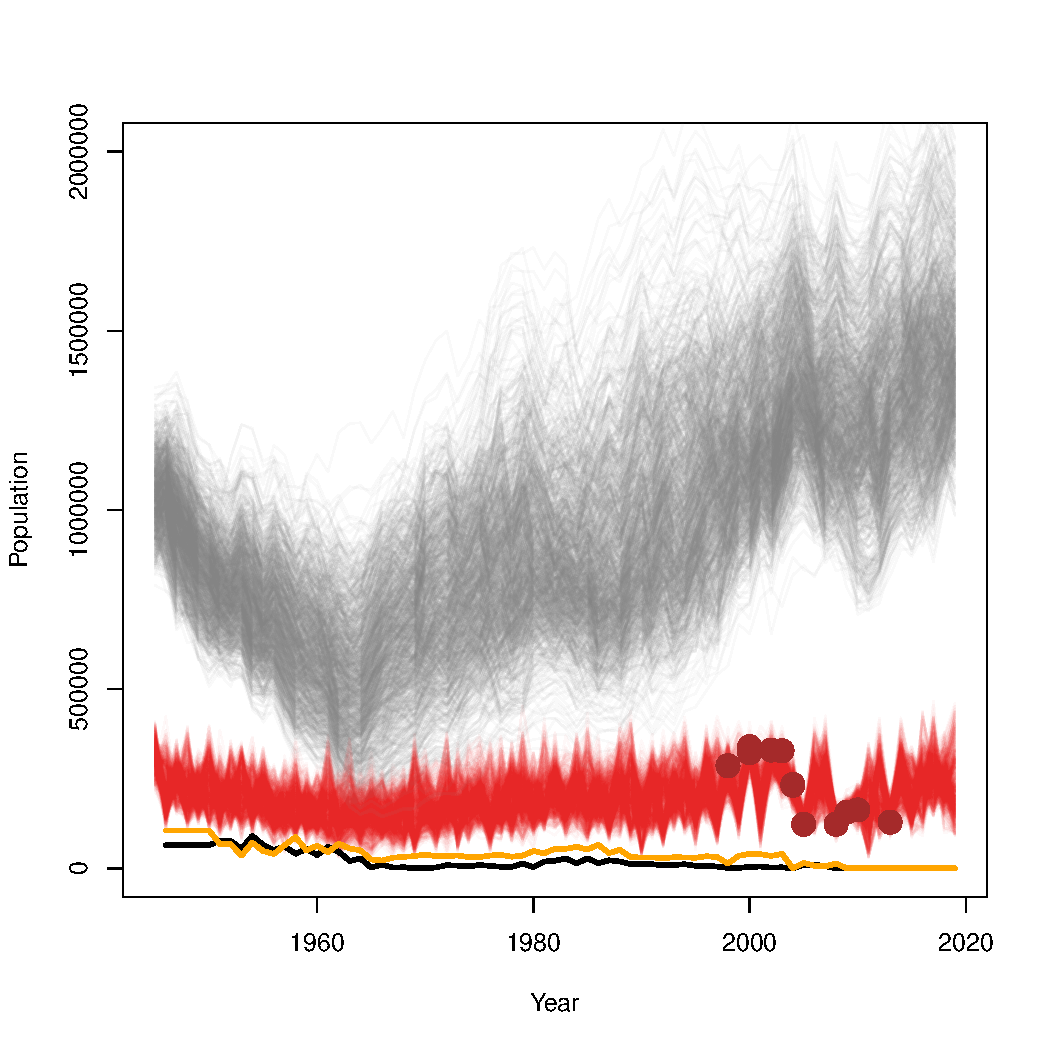
\includegraphics[height=6cm]{figure/Pop_traj} &
  \vspace{-5cm}
  \begin{itemize}
   {\tiny
   \item grey lines = 1000 posterior samples of adult abundance
   \item red lines = 1000 posterior samples of pup abundance
   \item brown dots = estimated pup abundance from surveys
   \item black line = adult harvest 
   \item orange line = pup harvest \\
   {} 
   }
  \end{itemize}
  
  \end{tabular}

\end{frame}

%-----------------------------------------------------------------------
%           Posterior phi
%-----------------------------------------------------------------------

\begin{frame} 
Posterior of phi (fecundity)
	\begin{tabular} {p{7cm} p{2cm}}

	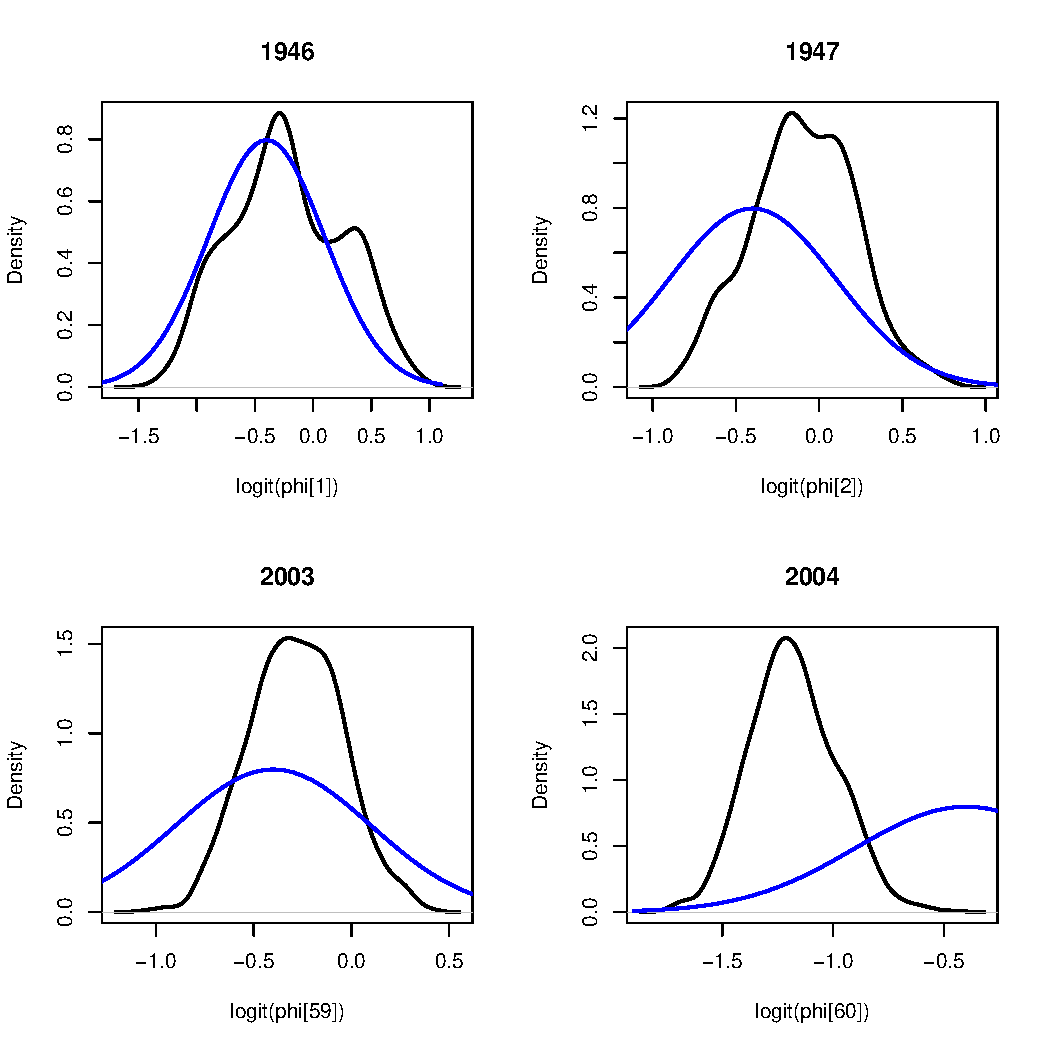
\includegraphics[height=7cm]{figure/Post_phi}  &

  \vspace{-5cm}
  \begin{itemize}
   {\tiny
   \item blue lines = prior
   \item black lines = posterior \\
   {} 
   }
  \end{itemize}
  \end{tabular}
\end{frame}

%-----------------------------------------------------------------------
%           Posterior delta
%-----------------------------------------------------------------------

\begin{frame} 

Posterior of delta (adult survival)
	\begin{tabular} {p{7cm} p{2cm}}

	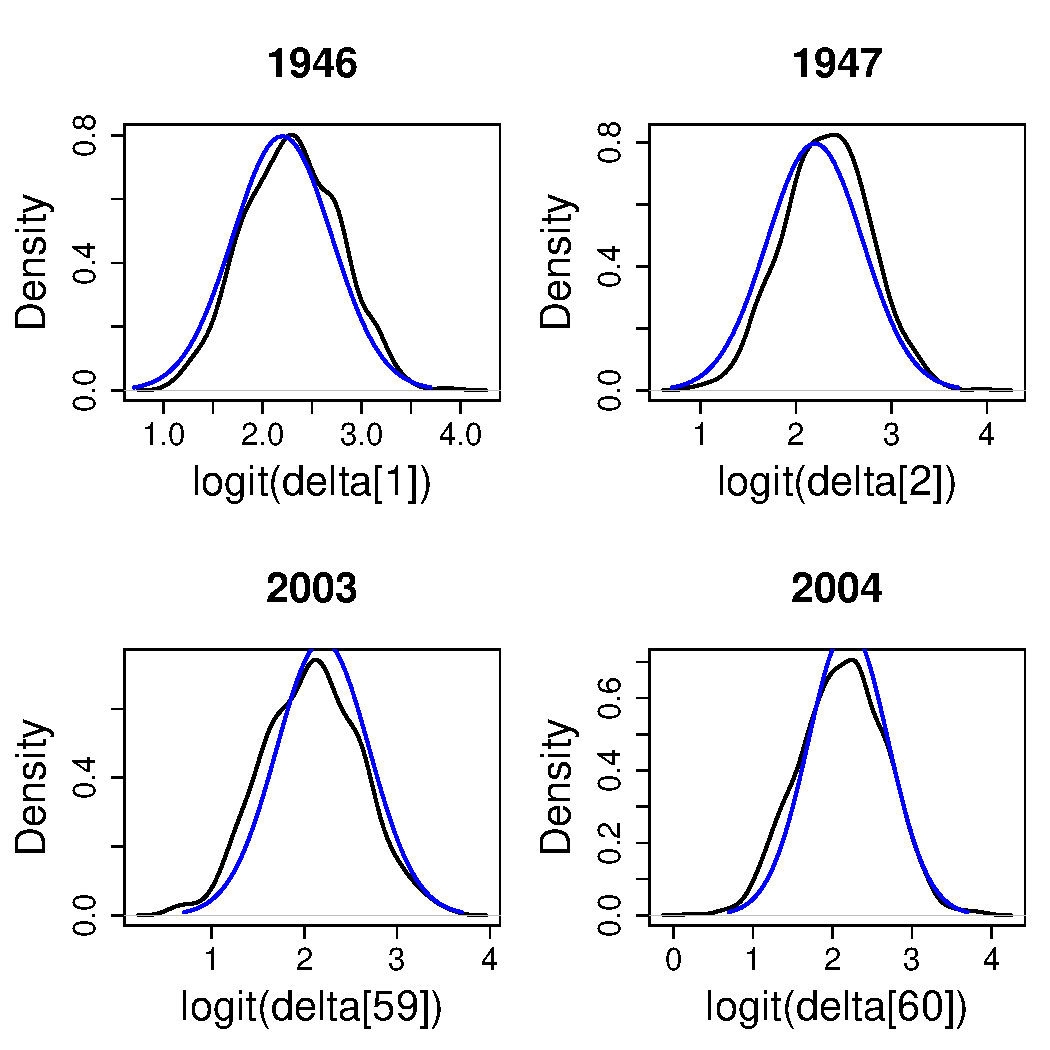
\includegraphics[height=7cm]{figure/Post_delta}  &

  \vspace{-5cm}
  \begin{itemize}
   {\tiny
   \item blue lines = prior
   \item black lines = posterior \\
   {} 
   }
  \end{itemize}
  \end{tabular}
\end{frame}


%-----------------------------------------------------------------------
%           Posterior kappa
%-----------------------------------------------------------------------

\begin{frame} 

Posterior of kappa (pup survival after surveys)
	\begin{tabular} {p{7cm} p{2cm}}

	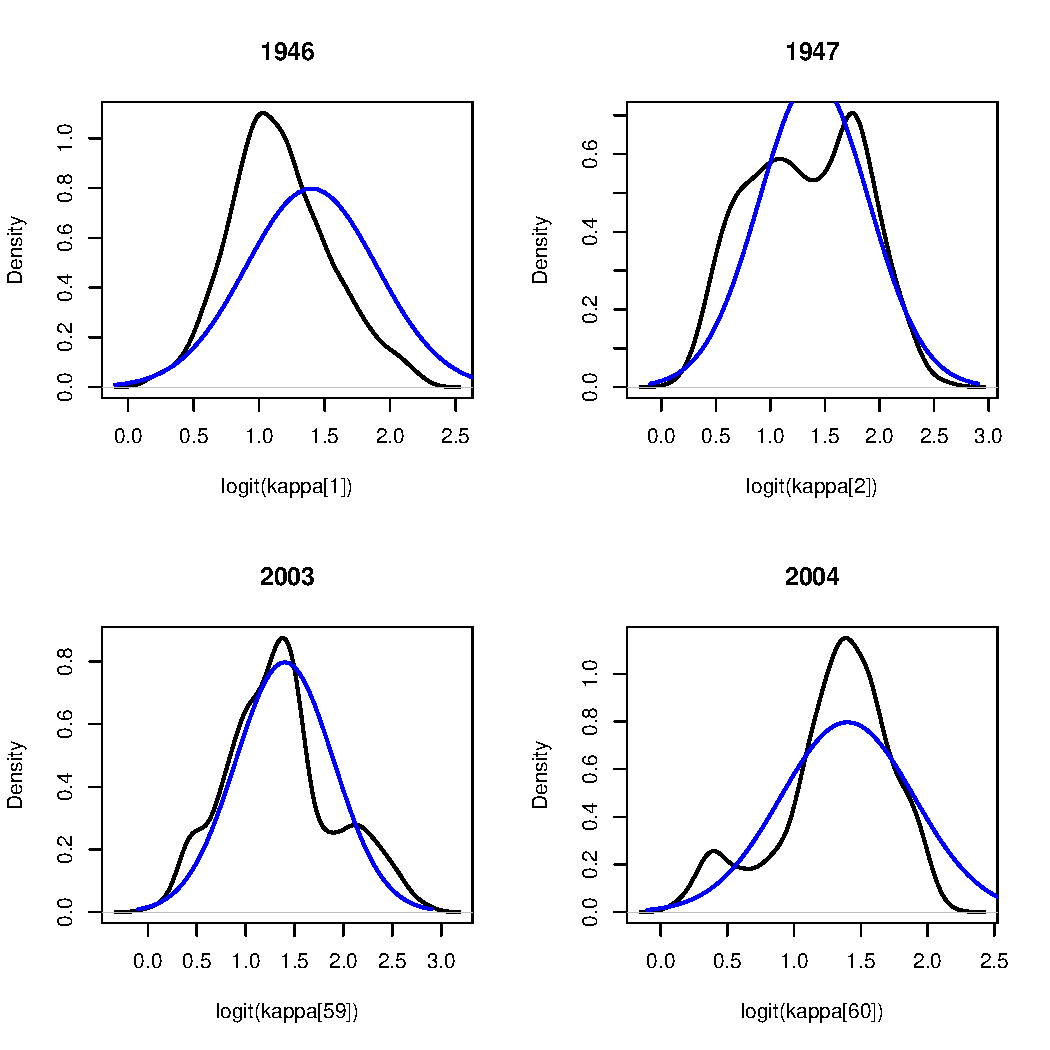
\includegraphics[height=7cm]{figure/Post_kappa}  &

  \vspace{-5cm}
  \begin{itemize}
   {\tiny
   \item blue lines = prior
   \item black lines = posterior \\
   {} 
   }
  \end{itemize}
  \end{tabular}
\end{frame}

%-----------------------------------------------------------------------
%           Posterior rho
%-----------------------------------------------------------------------

\begin{frame} 

Posterior of rho (controls fecundity decay with increased abundance)
	\begin{tabular} {p{7cm} p{2cm}}

	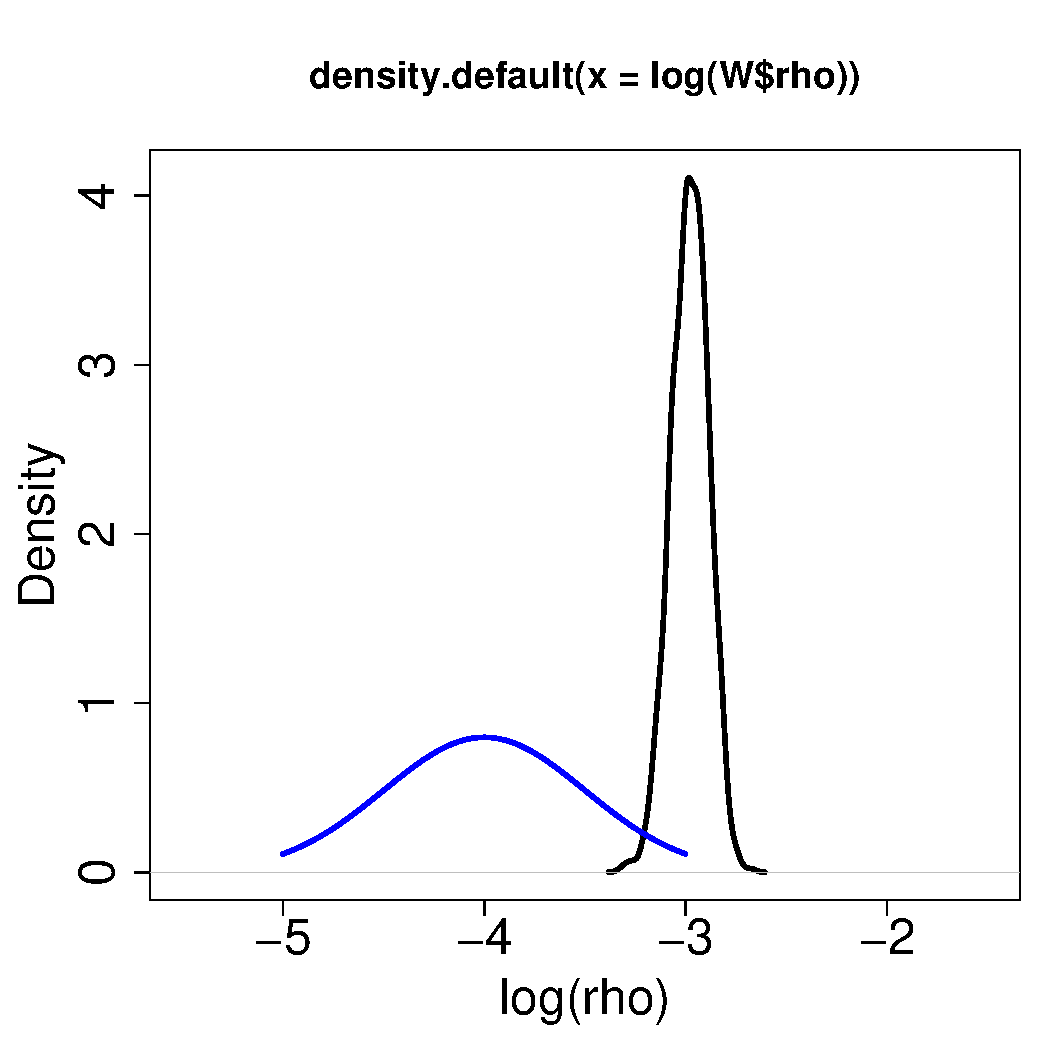
\includegraphics[height=6cm]{figure/Post_rho}  &

  \vspace{-5cm}
  \begin{itemize}
   {\tiny
   \item blue lines = prior
   \item black lines = posterior \\
   {} 
   }
  \end{itemize}
  \end{tabular}
\end{frame}


%-----------------------------------------------------------------------
%           Posterior Eigenvalues
%-----------------------------------------------------------------------

\begin{frame} 
Posterior of first eigenvalue

\begin{center}
	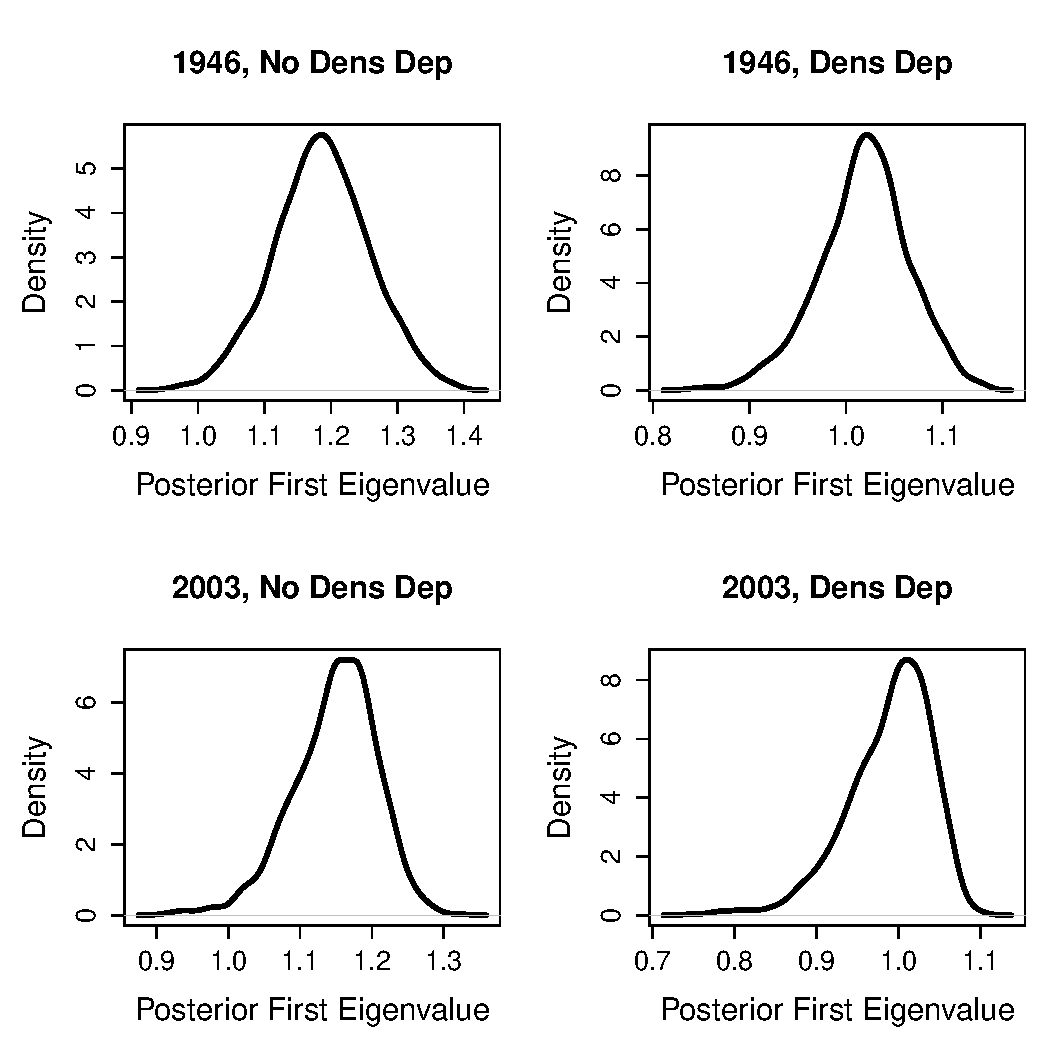
\includegraphics[height=7cm]{figure/Post_eigval} 
\end{center}
\end{frame}


%-----------------------------------------------------------------------
%           Notes
%-----------------------------------------------------------------------

\begin{frame}
Notes

\begin{itemize}

  \item The 2-age Leslie matrix model can be obtained from more detailed age- and sex-structured Leslie matrix models if they are collapsed properly.  The details can be found in the appendix of Boveng et al. (2018), listed above.  The intrinsic growth rate (first eigenvalue) and stable age proportions can be preserved between the detailed Leslie matrix and a collapsed Leslie matrix.  Collapsing the Leslie matrix model matches more closely to the data at hand.
       
\end{itemize}

\end{frame}

%-----------------------------------------------------------------------
%           Notes
%-----------------------------------------------------------------------

\begin{frame}

\begin{itemize}

  \item This is not a realistic model for the harpeast data, as there are better priors that can be developed from auxilliary data.  However, the results are intermediate to the State-space model (black line) and ICES management model (gray line) found in {{\O}ig{\aa}rd and Skaug}, ICES, 2015, but captures a decline in early years (See left Figure below).

\end{itemize}

\begin{center}
	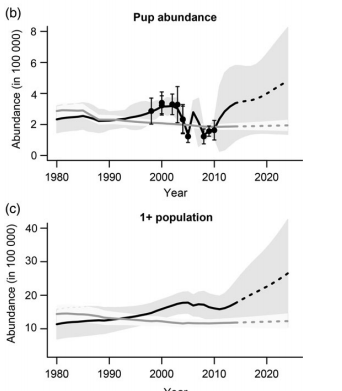
\includegraphics[height=3.5cm]{figure/Tor-Arne_ICES_2015_figure2.png}
  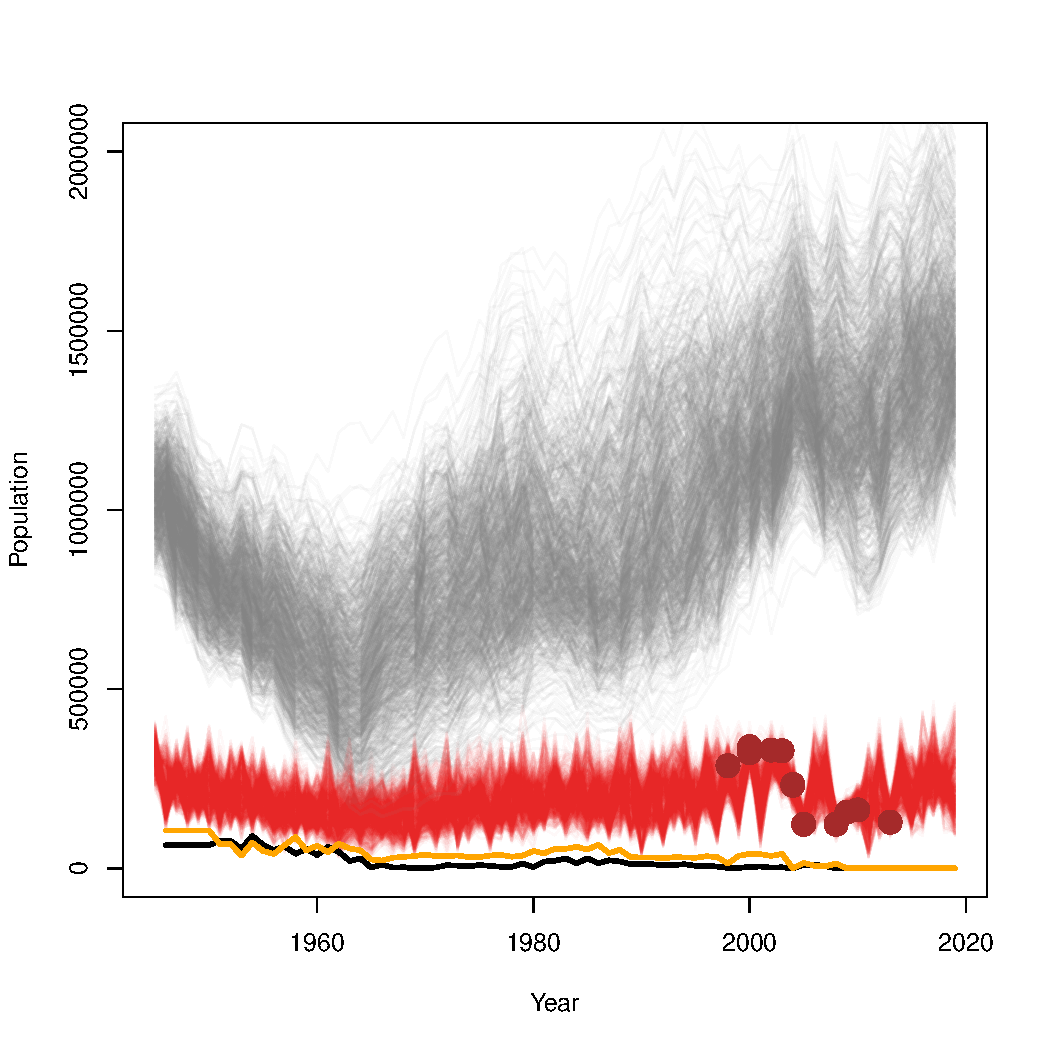
\includegraphics[height=3.5cm]{figure/Pop_traj} 
\end{center}

\end{frame}
%-----------------------------------------------------------------------
%           Notes
%-----------------------------------------------------------------------

\begin{frame}

\begin{itemize}
 
  \item The code runs quickly for such a small data set, even though there are 228 parameters (75 each for $\bdelta$, $\bkappa$, and $\bphi$, along with $\rho$, $P_{1}$, and $A_{1}$), by using batch sampling for $\bdelta$, $\bkappa$, and $\bphi$.

  \item With the high levels of harvest early on, if demographic parameters are drawn from a common distribution across years, the population decreases before recovering when harvest decreases.
  
  \item There appears to be information in the data on the density-dependent decay parameter controlling fecundity, at least given priors for all other parameters, as the posterior is substantially shifted from the prior.

\end{itemize}

\end{frame}

%-----------------------------------------------------------------------
%           Notes
%-----------------------------------------------------------------------

\begin{frame}

\begin{itemize}
 
  \item There is very little survey data, on pups only.  The results of the model depend a lot on the priors.  Many more prior scenarios can be tried with the R package.

  \item The attraction of a full Bayesian model is that we sample from the full joint posterior distribution.  The posterior distribution of pup and nonpup abundance is derived from the Leslie matrix model through the joint distribution of $\bdelta$, $\bkappa$, $\bphi$, $\rho$, $P_{1}$, and $A_{1}$.  Moreover, the posterior distribution of intrinsic growth, obtained from the first eigenvalue of the Leslie matrix model, is easily obtained if we have the joint posterior distribution of Leslie matrix parameters.
 
\end{itemize}

\end{frame}


%%%%%%%%%%%%%%%%%%%%%%%%%%%%%%%%%%%%%%%%%%%%%%%%%%%%%%%%%%%%%%%%%%%%%%%%%%%%%%%%%%
%%%%%%%%%%%%%%%%%%%%%%%%%%%%%%%%%%%%%%%%%%%%%%%%%%%%%%%%%%%%%%%%%%%%%%%%%%%%%%%%%%
%%%%%%%%%%%            %%%%%%%    %%%%%%%%  %%%%%%%       %%%%%%%%%%%%%%%%%%%%%%%%
%%%%%%%%%%%  %%%%%%%%%%%%%%%%%  %  %%%%%%%  %%%%%%%  %%%%  %%%%%%%%%%%%%%%%%%%%%%%
%%%%%%%%%%%  %%%%%%%%%%%%%%%%%  %%  %%%%%%  %%%%%%%  %%%%%%  %%%%%%%%%%%%%%%%%%%%%
%%%%%%%%%%%  %%%%%%%%%%%%%%%%%  %%%  %%%%%  %%%%%%%  %%%%%%%   %%%%%%%%%%%%%%%%%%%
%%%%%%%%%%%            %%%%%%%  %%%%  %%%%  %%%%%%%  %%%%%%%%  %%%%%%%%%%%%%%%%%%%
%%%%%%%%%%%  %%%%%%%%%%%%%%%%%  %%%%%  %%%  %%%%%%%  %%%%%%%   %%%%%%%%%%%%%%%%%%%
%%%%%%%%%%%  %%%%%%%%%%%%%%%%%  %%%%%%  %%  %%%%%%%  %%%%%%  %%%%%%%%%%%%%%%%%%%%%
%%%%%%%%%%%  %%%%%%%%%%%%%%%%%  %%%%%%%  %  %%%%%%%  %%%%  %%%%%%%%%%%%%%%%%%%%%%%
%%%%%%%%%%%            %%%%%%%  %%%%%%%%    %%%%%%%       %%%%%%%%%%%%%%%%%%%%%%%%
%%%%%%%%%%%%%%%%%%%%%%%%%%%%%%%%%%%%%%%%%%%%%%%%%%%%%%%%%%%%%%%%%%%%%%%%%%%%%%%%%%
%%%%%%%%%%%%%%%%%%%%%%%%%%%%%%%%%%%%%%%%%%%%%%%%%%%%%%%%%%%%%%%%%%%%%%%%%%%%%%%%%%


\end{document} 
